% 2012 年陕西卷文科第 18 题：直三棱柱 ABC-A1B1C1，∠CAB=90°。
% 来源 PDF：普通高考/2012/2012陕西文.pdf，第 2 页（印面 766）第 1 栏。
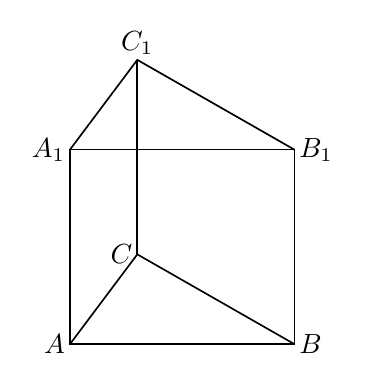
\begin{tikzpicture}[scale=0.95, semithick, every node/.style={inner sep=1.5pt}]
  \coordinate (A) at (0,0);
  \coordinate (B) at (3.0,0);
  \coordinate (C) at (0.9,1.2);
  \coordinate (A1) at (0,2.6);
  \coordinate (B1) at (3.0,2.6);
  \coordinate (C1) at (0.9,3.8);
  \draw (A) -- (B) -- (B1) -- (A1) -- cycle;
  \draw (A1) -- (C1) -- (B1);
  \draw (C) -- (C1);
  \draw (A) -- (C);
  \draw (B) -- (C);
  \draw[dashed] (A1) -- (B1);
  \node[left] at (A) {$A$};
  \node[right] at (B) {$B$};
  \node[left] at (C) {$C$};
  \node[left] at (A1) {$A_1$};
  \node[right] at (B1) {$B_1$};
  \node[above] at (C1) {$C_1$};
\end{tikzpicture}
